%\chapterauthor{Author Name}{Author Affiliation}
%\chapterauthor{Second Author}{Second Author Affiliation}
\chapter{Derivative}

Consider a continuous function $f(x)$ defined in $\left[a,b\right]$. In this chapter the ratio of change of $f(x)$ versus $x$ is quantitively derived and studied.

\section{A Motivating Example}

Consider the following motivating example.

\begin{shortbox}
\Boxhead{A Motivating Example}

Consider
\begin{eqnarray}
  y = f(x) = \left(|x|-1\right)^2. \label{ch2eq:motivatingexamplefx}
\end{eqnarray}
Obviously the above function \eqref{ch2eq:motivatingexamplefx} is continuous in $x\in\mathbb{R}$. We want to study the change $\Delta y = f\left(x+\Delta x\right) - f(x)$ given a small deviation $\Delta x$ at different values of $x$.

Q1: Describe $\Delta y$ given a small deviation $\Delta x$ at $x=2$, and describe the ratio $\frac{\Delta y}{\Delta x}$ when $\Delta x \rightarrow 0$.

Q2: Describe $\Delta y$ given a small deviation $\Delta x$ at $x=0$, and describe the ratio $\frac{\Delta y}{\Delta x}$ when $\Delta x \rightarrow 0$.

Q3: Describe the ratio $\frac{\Delta y}{\Delta x}$ at any $x$ when $\Delta x \rightarrow 0$.
\end{shortbox}

As a first step, plot $y$ as a function of $x$ from \eqref{ch2eq:motivatingexamplefx} in Fig.\ref{ch2fig:fxsimpleexample} for convenient analysis.
\begin{figure}
\centering
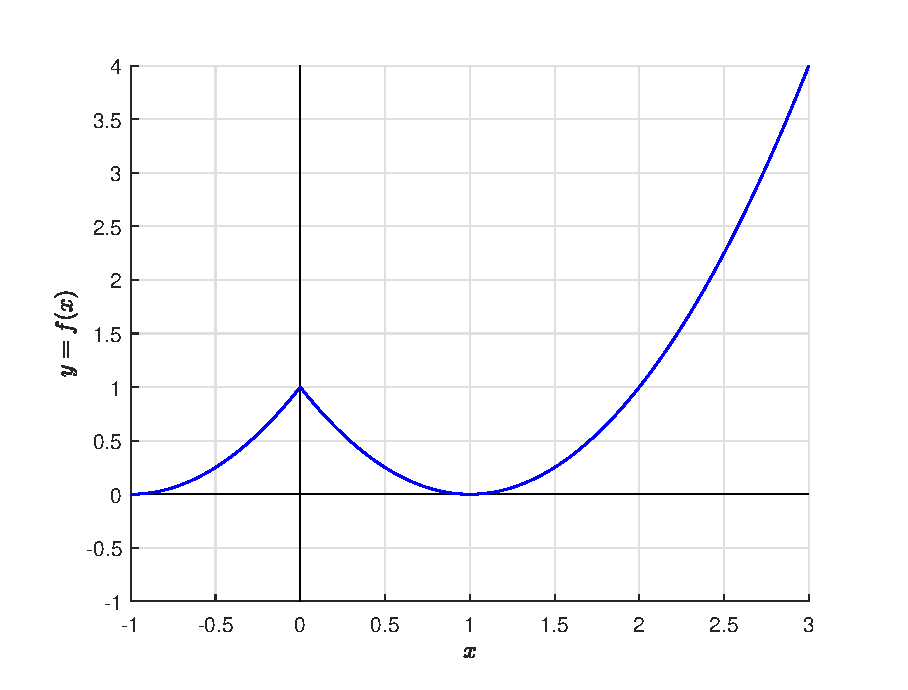
\includegraphics[width=250pt]{chapters/part-1/figures/fig_derivative_motiexp.eps}
\caption{Plot of $y$ as a function of $x$ in the motivating example.} \label{ch2fig:fxsimpleexample}
\end{figure}

Consider $x=2$. Variable $\Delta y = f\left(x+\Delta x\right) - f(x)$ is given in \eqref{ch2eq:deltayq1}. Notice that the deviation $\Delta x$ is supposed to be small, i.e. $|\Delta x| \approx 0$. Therefore, we can safely assume $2 + \Delta x \geq 0$ for simplicity.
\begin{eqnarray}
  \Delta y = f\left(2+\Delta x\right) - f(2)
  = \left(2 + \Delta x - 1\right)^2 - (2 - 1)^2
  = 2\Delta x + \Delta x^2. \label{ch2eq:deltayq1}
\end{eqnarray}

With \eqref{ch2eq:deltayq1}, it is possible to calculate $y$ at $x = 2 + \Delta x$ by using $y = f(2) + \Delta y$ for small $\Delta x$. For example, to calculate $f(1.9)$, substituting $\Delta x = -0.1$ into \eqref{ch2eq:deltayq1} gives $\Delta y = -0.19$, thus $f(1.9) = f(2) - 0.19 = 0.81$.

From \eqref{ch2eq:deltayq1}, the ratio $\frac{\Delta y}{\Delta x}$ can be calculated as
\begin{eqnarray}
  \left.\dfrac{\Delta y}{\Delta x}\right|_{x=2} &=& 2 + \Delta x, \label{ch2eq:secantexpression}
\end{eqnarray}
where $(\cdot)|_{x=a}$ represents substituting $x=a$ into $(\cdot)$.

Notice that \eqref{ch2eq:secantexpression} can be interpreted geometrically as the slope of secant of $(2,1)$ and $(x+\Delta x, f\left(x+\Delta x)\right)$. For example, when $\Delta x = 0.5$, the slope of secant $(2,1)$ and $(2.5,2.25)$ can be obtained using \eqref{ch2eq:secantexpression} as $2.5$, which is shown as the red solid line in Fig. \ref{ch2fig:simpleexptangent}.
\begin{figure}
\centering
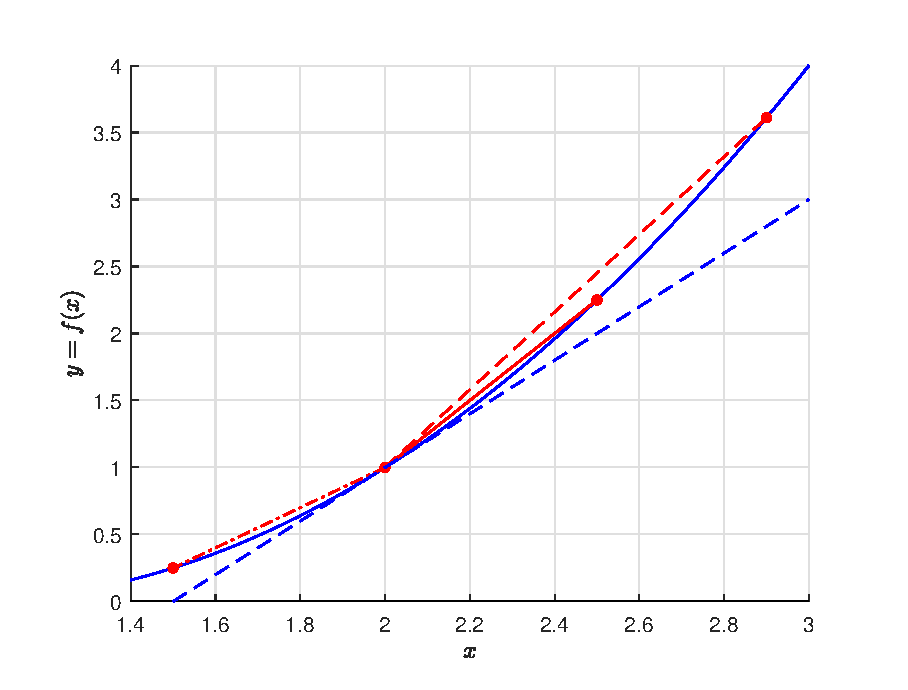
\includegraphics[width=250pt]{chapters/part-1/figures/fig_simpleexp_tangent.eps}
\caption{Slope of secant and tangent of $y=f(x)$ at $x=2$.} \label{ch2fig:simpleexptangent}
\end{figure}
Other two examples when $\Delta x= 0.9$ and $\Delta x = -0.5$ are given by red dashed line and red dot-dashed line in Fig. \ref{ch2fig:simpleexptangent} respectively, and their slopes can be calculated as $2.9$ and $1.5$ respectively using \eqref{ch2eq:secantexpression}.

Apparently, the slope of the secant depends on $\Delta x$, which can be seen from both equation \eqref{ch2eq:secantexpression} and Fig. \ref{ch2fig:simpleexptangent}. From the figure, when $\Delta x \rightarrow 0$, the slope of the tangent at $x=2$ can be obtained, as given by the blue dashed line in Fig. \ref{ch2fig:simpleexptangent}. From \eqref{ch2eq:secantexpression},
\begin{eqnarray}
  \lim_{\Delta x \rightarrow 0} \left.\dfrac{\Delta y}{\Delta x}\right|_{x=2} &=& 2 \label{ch2eq:simpleexampleratioxtwo}
\end{eqnarray}
which is the slope of the tangent of $y=f(x)$ at $x=2$.

Consider $x=0$. Variable $\Delta y = f\left(x+\Delta x\right) - f(x)$ can be obtained as given in \eqref{ch2eq:deltayq2}. Different from \eqref{ch2eq:deltayq1}, this time the analytical equation has two forms, depending on the sign of $\Delta x$.
\begin{eqnarray}
  \Delta y = f\left(\Delta x\right) - f(0) = \left\{\begin{array}{cc}
                                                      \Delta x^2 - 2\Delta x & \Delta x > 0 \\
                                                      \Delta x^2 + 2\Delta x & \Delta x < 0
                                                    \end{array}\right.. \label{ch2eq:deltayq2}
\end{eqnarray}
From \eqref{ch2eq:deltayq2}, the ratio $\frac{\Delta y}{\Delta x}$ can be calculated as
\begin{eqnarray}
  \left.\dfrac{\Delta y}{\Delta x}\right|_{x=0} &=& \left\{\begin{array}{cc}
                                          -2 + \Delta x & \Delta x > 0 \\
                                          2 + \Delta x & \Delta x < 0
                                        \end{array}\right.. \label{ch2eq:deltayq2ratio}
\end{eqnarray}
Equation \eqref{ch2eq:deltayq2ratio} implies that
\begin{eqnarray}
  \lim_{\Delta x\rightarrow 0^-} \left.\dfrac{\Delta y}{\Delta x}\right|_{x=0} &=& 2, \nonumber \\
  \lim_{\Delta x\rightarrow 0^+} \left.\dfrac{\Delta y}{\Delta x}\right|_{x=0} &=& -2, \nonumber
\end{eqnarray}
and $\lim_{\Delta x\rightarrow 0}\left.\frac{\Delta y}{\Delta x}\right|_{x=0}$ does not exist. This can be intuitively comprehended from Fig. \ref{ch2fig:fxsimpleexample} as there is no tangent for the curve at $x=0$.

Consider Q3. From what have been achieved in Q1 and Q2, we know that at different value of $x$, the ratio $\lim_{\Delta x\rightarrow 0}\frac{\Delta y}{\Delta x}$ can be different. In this example, we need to discuss three sub-cases $x<0$, $x=0$ and $x>0$. Notice that since $\Delta x$ is small ($\Delta x \rightarrow 0$ is studied), we assume $x + \Delta x$ has the same sign with $x$ when $x\neq 0$.

When $x<0$,
\begin{eqnarray}
% \nonumber % Remove numbering (before each equation)
  \Delta y &=& f\left(x + \Delta x\right) - f(x) \nonumber \\
   &=& \left(-x - \Delta x - 1\right)^2 - \left(-x - 1\right)^2 \nonumber \\
   &=& \Delta x^2 + 2x\Delta x + 2\Delta x, \nonumber
\end{eqnarray}
and the ratio is
\begin{eqnarray}
  \dfrac{\Delta y}{\Delta x} &=& \Delta x + 2x + 2. \nonumber
\end{eqnarray}
Thus,
\begin{eqnarray}
% \nonumber % Remove numbering (before each equation)
  \lim_{\Delta x\rightarrow 0} \dfrac{\Delta y}{\Delta x} &=& 2x + 2 \label{ch2eq:simpleexpratio1}
\end{eqnarray}

When $x=0$, as discussed previously, $\lim_{x\rightarrow 0} \frac{\Delta y}{\Delta x}$ does not exist.

When $x>0$,
\begin{eqnarray}
% \nonumber % Remove numbering (before each equation)
  \Delta y &=& f\left(x + \Delta x\right) - f(x) \nonumber \\
   &=& \left(x + \Delta x - 1\right)^2 - \left(x - 1\right)^2 \nonumber \\
   &=& \Delta x^2 + 2x\Delta x - 2\Delta x, \nonumber
\end{eqnarray}
and the ratio is
\begin{eqnarray}
  \dfrac{\Delta y}{\Delta x} &=& \Delta x + 2x - 2. \nonumber
\end{eqnarray}
Thus,
\begin{eqnarray}
  \lim_{\Delta x\rightarrow 0} \dfrac{\Delta y}{\Delta x} &=& 2x - 2 \label{ch2eq:simpleexpratio2}
\end{eqnarray}

To summarize \eqref{ch2eq:simpleexpratio1} and \eqref{ch2eq:simpleexpratio2}
\begin{eqnarray}
  \lim_{\Delta x\rightarrow 0} \dfrac{\Delta y}{\Delta x} &=& \left\{\begin{array}{cc}
                                                                2x + 2 & x < 0 \\
                                                                2x - 2 & x > 0
                                                              \end{array}\right., \label{ch2eq:simpleexpgeneralratio}
\end{eqnarray}
which can be interpreted as the slope of tangent of curve $y=f(x)$ at different $x$ in Fig. \ref{ch2fig:fxsimpleexample}.

This motivating example shows that for a function $y=f(x)$, the ratio $\lim_{\Delta x \rightarrow 0}\frac{f(x + \Delta x)}{\Delta x}$ may change for different $x$, and sometimes may not even exist. The limit  $\lim_{\Delta x \rightarrow 0}\frac{f(x + \Delta x)}{\Delta x}$ itself is also a function of $x$, which we call \textit{the derivative of $f(x)$}.

\section{Derivative of a Function}

The formal definition of the derivative of a scalar function $f(x)$ with respect to $x$ is given as follows.

\begin{VF}
\textbf{Definition of the derivative of a function}:
\\
\\
\noindent The derivative of $f(x)$ at $x=a$, denoted by $f^\prime(a)$, is given as follows
\begin{eqnarray}
  f^\prime(a) &=& \lim_{\Delta x \rightarrow 0}\dfrac{f\left(a + \Delta x\right)-f(a)}{\Delta x} \label{ch2eq:definitionderivative}
\end{eqnarray}
if such limit in \eqref{ch2eq:definitionderivative} exists. In this case, $f(x)$ is called differentiable at $x=a$.
\\
\\
If $y=f(x)$, equation \eqref{ch2eq:definitionderivative} can also be written as
\begin{eqnarray}
% \nonumber % Remove numbering (before each equation)
  \left.\dfrac{dy}{dx}\right|_{x=a} &=& f^\prime(a), \nonumber
\end{eqnarray}
where $\frac{dy}{dx}$ can be taken as an alternative denotation of $f^\prime(x)$, and $\frac{d}{dx}$ is called the \textit{differentiation operator}.
\end{VF}

It is easy to prove that a necessary condition for a function $f(x)$ to be differentiable at $x=a$ is that $f(x)$ is continuous at $x=a$.

\section{Calculation of the Derivative of a Function}

The derivative of commonly seen functions are concluded in the following Table \ref{chi2table:commonderivative}.

\begin{table}
%\noautomaticrules
\tabletitle{Derivative of commonly seen functions.} \label{chi2table:commonderivative}
\begin{tabular}{lll}
\tch{$f(d)$} & \tch{$f^\prime(x)$} & Comments  \\ \hline
$c$ & $0$ & \\
$x^n$ & $nx^{n-1}$ & $n\neq0$ \\
$\textup{sin}(x)$ & $\textup{cos}(x)$ & \\
$\textup{cos}(x)$ & $-\textup{sin}(x)$ & \\
$a^x$ & $a^x\textup{ln}a$ & $a>0$ \\
$\textup{log}_ax$ & $\dfrac{1}{\textup{ln}a}\dfrac{1}{x}$ & $a, x > 0$ \\
\end{tabular}
\end{table}

As two very commonly seen special cases of $a^x$ and $\textup{log}_ax$ in Table \ref{chi2table:commonderivative},
\begin{eqnarray}
    \dfrac{d}{dx}e^x &=& e^x, \nonumber \\
    \dfrac{d}{dx}\textup{ln}x &=& \dfrac{1}{x}. \nonumber
\end{eqnarray}

With both $f_1(x)$ and $f_2(x)$ differentiable,
\begin{eqnarray}
     \dfrac{d}{dx}\left(af_1(x) + bf_2(x)\right) &=& a\dfrac{d}{dx}f_1(x) + b\dfrac{d}{dx}f_2(x), \nonumber \\
     \dfrac{d}{dx}\left(f_1(x)f_2(x)\right) &=& f_2(x)\dfrac{d}{dx}f_1(x) + f_1(x)\dfrac{d}{dx}f_2(x), \nonumber \\
     \dfrac{d}{dx}\left(\dfrac{f_1(x)}{f_2(x)}\right) &=& \dfrac{ f_2(x)\dfrac{d}{dx}f_1(x) - f_1(x)\dfrac{d}{dx}f_2(x)}{\left(\dfrac{d}{dx}f_2(x)\right)^2}. \nonumber
\end{eqnarray}

If $f = f(x)$ and $g = g(f)$, $\frac{dg}{dx}$ can be calculated using \textit{chain rule for composite function} as
\begin{eqnarray}
     \dfrac{dg}{dx} &=& \dfrac{d}{df}g(f)\dfrac{d}{dx}f(x). \nonumber
\end{eqnarray}
For example, if $f = 3x^2 - 2$ and $g = f^2$,
\begin{eqnarray}
     \dfrac{dg}{dx} = \dfrac{d}{df}g(f)\dfrac{d}{dx}f(x) = \left(2f\right)\left(6x\right) = 36x^3 - 24x. \nonumber
\end{eqnarray}

There are a bunch of theorems not covered with much details in this notebook. For example, the famous \textit{mean value theorem} says if a function $f(x)$ is continuous in $[a, b]$ and has a derivative everywhere in $(a, b)$, there must be such $a < c < b$ that
\begin{eqnarray}
     \dfrac{f(b)-f(a)}{b-a} &=& f^\prime(c). \nonumber
\end{eqnarray}
Some of these theorems are widely used in the derivation and proof of other theorems.
